\documentclass{article}
\usepackage{graphicx} % Required for inserting images
\usepackage[italian]{babel}
\usepackage[hidelinks]{hyperref}
\usepackage{todonotes}
\usepackage{biblatex}
\usepackage{listings}
\usepackage{parskip}

\title{
    Project Management \\
    \textbf{ 
        Estimates of the \\ 
        Required Resources \\ 
        for Web Application: \\
        \textit{Google CookBook}
    }
}
\author{
    Marica Pasquali \\ 
    (\href{mailto:marica.pasquali@studio.unibo.it}{marica.pasquali@studio.unibo.it})
}

\begin{document}

\maketitle
\newpage \tableofcontents \newpage

\section{Risorse Umane}

\begin{itemize}
    \item 1 Project Manager 
    \item 2 full stack developer senior 
    \item Developers junior
    \begin{itemize}
        \item 2 back-end developer
        \item 2 front-end developer
    \end{itemize} 
    \item 1 \href{https://en.wikipedia.org/wiki/Database_administrator}{database administrator (DBA)} 
\end{itemize}


\section{Equipaggiamento}


\begin{figure}[htbp]
    \centering
    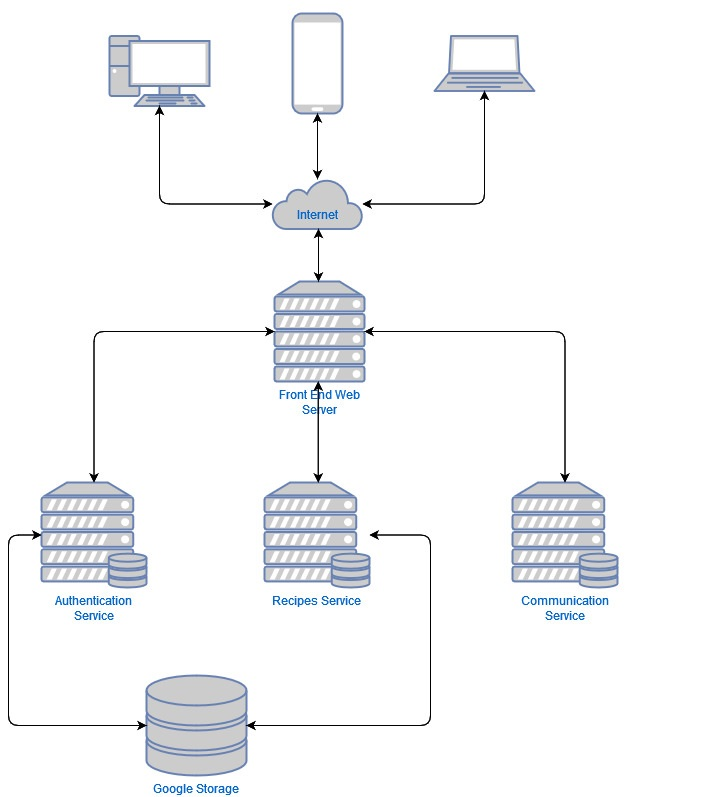
\includegraphics[scale=0.7]{./imgs/pm-architecture.jpg}
    \caption{Architettura}
\end{figure}

\subsection{Spazi in Cloud}
\begin{itemize}
    \item 1 server per Authentication Service
    \item 1 server per Recipes Service
    \item 1 server per Communication Service
    \item 1 web server di front-end
    \item 1 Storage offerto da Google
\end{itemize}

\subsection{Spazi in locale}
\begin{itemize}
    \item 1 server per il testing
    \item 1 database per il testing
\end{itemize}


\section{Materiale}
\begin{itemize}
    \item Software per la gestione dei task del progetto (ad esempio, Trello)
    \item Software per la modellazione degli schemi dei database (relazionale, documentale, a grafo)
    \item Software per la modellazione delle API dei vari servizi (ad esempio, SwaggerHub)
\end{itemize}


\section{Facilities}
\begin{itemize}
    \item 1 sala riunioni
    \item Lavagna
    \item Pennarelli
    \item Post-it
    \item Carte da poker
\end{itemize}


\end{document}